% !TEX TS-program = pdflatex
% !TEX encoding = UTF-8 Unicode

% This is a simple template for a LaTeX document using the "article" class.
% See "book", "report", "letter" for other types of document.

\documentclass[11pt]{report} % use larger type; default would be 10pt

\usepackage[utf8]{inputenc} % set input encoding (not needed with XeLaTeX)

%%% Examples of Article customizations
% These packages are optional, depending whether you want the features they provide.
% See the LaTeX Companion or other references for full information.

%%% PAGE DIMENSIONS
\usepackage{geometry} % to change the page dimensions
\geometry{a4paper} % or letterpaper (US) or a5paper or....
% \geometry{margin=2in} % for example, change the margins to 2 inches all round
% \geometry{landscape} % set up the page for landscape
%   read geometry.pdf for detailed page layout information

\usepackage{graphicx} % support the \includegraphics command and options

% \usepackage[parfill]{parskip} % Activate to begin paragraphs with an empty line rather than an indent

%%% PACKAGES
\usepackage{booktabs} % for much better looking tables
\usepackage{array} % for better arrays (eg matrices) in maths
\usepackage{paralist} % very flexible & customisable lists (eg. enumerate/itemize, etc.)
\usepackage{verbatim} % adds environment for commenting out blocks of text & for better verbatim
\usepackage{subfig} % make it possible to include more than one captioned figure/table in a single float
\usepackage{graphicx}
\usepackage{xcolor}
\usepackage{listings}
\lstset{basicstyle=\ttfamily,
  showstringspaces=false,
  commentstyle=\color{red},
  keywordstyle=\color{blue}
}

% These packages are all incorporated in the memoir class to one degree or another...

%%% HEADERS & FOOTERS
\usepackage{fancyhdr} % This should be set AFTER setting up the page geometry
\pagestyle{fancy} % options: empty , plain , fancy
\renewcommand{\headrulewidth}{0pt} % customise the layout...
\lhead{}\chead{}\rhead{}
\lfoot{}\cfoot{\thepage}\rfoot{}

%%% SECTION TITLE APPEARANCE
\usepackage{sectsty}
\usepackage{indentfirst}
\allsectionsfont{\sffamily\mdseries\upshape} % (See the fntguide.pdf for font help)
% (This matches ConTeXt defaults)

%%% ToC (table of contents) APPEARANCE
\usepackage[nottoc,notlof,notlot]{tocbibind} % Put the bibliography in the ToC
\usepackage[titles,subfigure]{tocloft} % Alter the style of the Table of Contents
\renewcommand{\cftsecfont}{\rmfamily\mdseries\upshape}
\renewcommand{\cftsecpagefont}{\rmfamily\mdseries\upshape} % No bold!

\makeatletter
\@addtoreset{section}{chapter}
\@addtoreset{subsection}{chapter}
\@addtoreset{subsubsection}{chapter}
\makeatother

%%% Font

%%% Spacing between paragraphs
\edef\restoreparindent{\parindent=\the\parindent\relax}
\usepackage{parskip}
\restoreparindent

%%% The "real" document content comes below...

\title{Supporting a Hadoop Cluster with Unused PCs}
\author{Floriane Le Floch - Arthur Busser - Paul Dennetiere}
%\date{} % Activate to display a given date or no date (if empty),
         % otherwise the current date is printed 

\begin{document}

\maketitle
\renewcommand{\contentsname}{Summary}
\newpage
\tableofcontents
\newpage

\part{Introduction}

\section{Personal computers}
In 2008, approximately 1 billion personal computers were in use worldwide. Today, that number stands above 2 billion\footnote{Source: Forrester Research}. In the United States of America, Japan, Germany, the United Kingdom, France, and Italy, the number of PCs gets closer to the number of inhabitants every year\footnote{Source: Computer Industry Almanac Inc.}.

In 2016, more than half (50.1\%) of the world's population was an Internet user\footnote{Source: http://www.internetworldstats.com/}. In this Information Age, most computers are connected to each other and can easily communicate. Countless companies rely on computers for communication, marketing, accounting, storage, documents and reports, education, and research.

As things stand, personal computers used for work and/or personal activities add up to an immense amount of processing power and that amount is growing continuously.

\section{The problem}
Very few people use the full computing capabilities of their PCs. Even then, there are long periods of time every day when PCs are left unused. In many companies, almost every employee is provided with a PC. At night, desktop computers - and laptops too - are often left on, staying idle until their user returns in the morning. During this time, those PCs could be doing something.

The main problem with personal computers is that they are personal. The average person will never use the full potential of their PC, simply because most of the time they will not be using it. This results in a huge amount of processing power going to waste. If only the computer's capabilities could be shared somehow...
  
\section{Our idea}
As we stated above, most computers are connected and can easily communicate with each other. Many professionals have used this to their advantage, organizing computers into clusters that could tackle computation problems as a whole.

Our idea is to create a tool that, once installed on a personal computer, would wait for the PC to be unused to connect it to a remote computer cluster. The cluster could then use the new node's processing power to advance in its current calculations. When the PC would once again need to be used, it would disconnect from the cluster and continue as it normally does.

\part{Our solution}
\vspace*{\stretch{1}}
We want to make unused computers available for a Hadoop Cluster. In order to do that, we want to check at regular intervals if a computer is used or not (i.e. is in sleep mode). Our goal is to dynamically add sleeping computer to the cluster, in order to make more resources available.

In order to achieve this, we will have to ensure several things. This part will deal with the general structure, and what this structure induces for the cluster and added computers.
\vspace*{\stretch{1}}

\chapter{Setting up a DataNode on an unused computer}
First we will have to make the computer we want to add able to communicate with the Master (NameNode). We have several options to achieve this: \begin{itemize}
\item Virtualization
\item Use only linux distributions
\item Application containers
\end{itemize}
Only using linux distributions will greatly impact the interest of this project, so it is clearly not a solution. Virtualization does not seem good either, because of its need of resources, and the general weight of those solutions. That is why we will use an Application Container: Docker.

\section{Docker}
Docker defines itself as: \begin{quote}"Docker containers wrap up a piece of software in a complete filesystem that contains everything it needs to run: code, runtime, system tools, system libraries – anything you can install on a server. This guarantees that it will always run the same, regardless of the environment it is running in."\end{quote}

Therefore by using Docker we will be able to use a linux application on every operating system encountered in the company.
Moreover, by doing a snapshot of a running configuration, Docker allows us to deploy a solution very easily, and with a good velocity.
Finally, the global strategy is to have a "Slave Image" for Docker:
Every computer in the company will have Docker installed on it, and will start the Docker application every time the computer goes in sleep mode (we can easily do this through a C\# script, running in background, checking the sleep mode, and launching the Docker application, or even using TaskLauncher included in Microsoft's OS).

\begin{figure}[ht!]
\centering
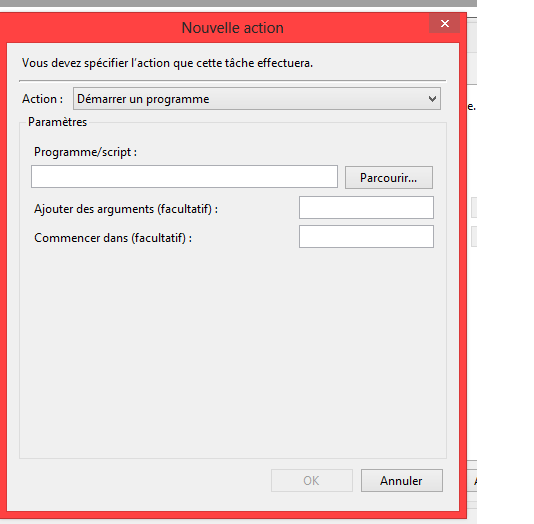
\includegraphics[width=90mm]{screen.png}
\caption{Screen capture of Microsoft's Task Launcher \label{overflow}}
\end{figure}

\section{Configuration}
We supposed that a "classical Hadoop cluster" is already configured (meaning we do not install a full cluster). So our goal is to provide a Hadoop slave service on the computer, and to make it communicate with the Master.

We will first create an image of a running configuration. Such images are already available on Docker's Hub (Docker's image sharing website), but we will assume that we can not get such images: 
The first thing to do is to create a linux distribution image, a Debian for example. After that we install the Hadoop slave service on this Debian.

\begin{itemize}
\item Creating Hadoop user and password: 

\begin{lstlisting}[language=bash]
useradd hadoop
passwd hadoop
\end{lstlisting}

\item Install Slave service on all slave by running on Master :
\begin{lstlisting}[language=bash]
# su hadoop 
$ cd /opt/hadoop 
$ scp -r hadoop hadoop-slave-1:/opt/hadoop 
$ scp -r hadoop hadoop-slave-2:/opt/hadoop
\end{lstlisting}
\item Setup password-less connectivity from master to new slave.
\begin{lstlisting}[language=bash]
mkdir -p $HOME/.ssh 
chmod 700 $HOME/.ssh 
ssh-keygen -t rsa -P '' -f $HOME/.ssh/id_rsa 
cat $HOME/.ssh/id_rsa.pub >> $HOME/.ssh/authorized_keys 
chmod 644 $HOME/.ssh/authorized_keys
scp $HOME/.ssh/id_rsa.pub hadoop@IPPATH:/home/hadoop/
\end{lstlisting}
Where IPPATH is the IP address of the new node.
Do the same thing on the slaves, in order to exchange ssh keys between master and slaves.

\item Then set a Hostname on new slaves in  /etc/sysconfig/network:
\begin{lstlisting}[language=bash]
NETWORKING=yes 
HOSTNAME=slaveX.in
\end{lstlisting}
Where X is the node Id (arbitrarily set, but unique)

\item Run on every new slave the following, to make changes effective: 
\begin{lstlisting}[language=bash]
hostname slaveX.in
\end{lstlisting}

\item Update /etc/hosts on all machines of the cluster with the following lines:
\begin{lstlisting}[language=bash]
IPPATH slaveX.in slaveX
\end{lstlisting}
\end{itemize}
By using this configuration we are able to dynamically add a data node to an existing cluster. The only point of failure is on IP addresses: every node should have a different one, and use it in order to have a functional network. However, this IP address can be found on the host.

Finally, the new slave has to start HDFS by using this command:
\begin{lstlisting}[language=bash]
./bin/hadoop-daemon.sh start datanode
\end{lstlisting}
This last command will have to be executed every time the Docker application is started.

\section{Conclusion}
In conclusion, docker is a tool (application container) that will allow us to run Hadoop on nearly every system, as well as allow us to have a configuration routine that practically does not differ from one machine to another. By porting this solution on every computer in the company, we can assume that every computer going in sleep mode, having a Docker image configured like above, will connect to the master, and be part of the Hadoop cluster.

However we can easily imagine that many difficulties will come up, and we will discuss them below.

\part{Difficulties that we expect to encounter}
\chapter{Redundancy Problems}
\section{What we expect to happen}
Because of bla bla blabla bla blabla bla blabla bla blabla bla blabla bla blabla bla blabla bla blabla bla blabla bla blabla bla bla

\end{document}
